\section{Experimental Results}
\subsection{Methodology}

%We study HM in a machine with two memory nodes. We use one as fast local memory and one as slow remote memory. Table~\ref{tab:hardware} summarizes the hardware we use. %for evaluation. %We inject traffic by using memhog inject traffic to change the bandwidth of slow memory.

%\textcolor{green}{We implement \name in Linux v4.9 and TensorFlow v1.14. The kernel change is for profiling and the Tesorslow change is for runtime page migration. The statistics of kernel modification given by git diff is X; the statistic of TensorFlow source code modification given by git diff is X.}



%\textcolor{green}{We evaluate 5 DNN models to verify the effectiveness of \name. Table~\ref{tab:models} shows the detail information. We use the implemetation of ResNet\_v2-152, LSTM, and Wide\_Deep model from TensorFlow software package~\cite{tf_models}, ResNet-32 from ~\cite{dcgan} and DCGAN from~\cite{resnet_32}.  The default intra-op and inter-op parallelisms are set as the number of one socket physical cores of the hardware platform (24 on the experimental platform).}

We study HM in a machine with two memory nodes. We use one as fast local memory and one as slow remote memory. Table~\ref{tab:hardware} summarizes the hardware we use. We evaluate five DNN models.
%to verify the effectiveness of \name. 
Table~\ref{tab:models} shows model details. For %ResNet\_v2-152, LSTM, and %Wide\_Deep 
LSTM and MobileNet models in our evaluation, we use the implementations from TensorFlow~\cite{tf_models}; For ResNet, BERT and DCGAN, we use~\cite{resnet_32}, ~\cite{bert_github} and~\cite{dcgan} respectively. 
We train BERT with five datasets from GLUE~\cite{wang-etal-2018-glue}  shown in Table~\ref{tab:glue_bench}. \textcolor{check}{We present average results of the five datasets in this section to save space}. To use TensorFlow, the intra-op parallelism (i.e., the number of threads to run an operation) and inter-op parallelism (i.e., the maximum number of operations to co-run) are set as 24, which is the number of physical cores in a socket in our platform. 

We compare \name with a state-of-the-art page migration system from Yan et al.~\cite{Yan:ASPLOS19}. They introduce a page migration algorithm by improving an existing page replacement mechanism in the Linux kernel (i.e., an FIFO-based active list~\cite{Yan:ASPLOS19}, named \textit{improved active list} (IAL) in the following discussion). In~\cite{Yan:ASPLOS19}, they improve the performance of the page migration mechanism by using four threads for parallel page copying and eight threads for concurrent page migration, and they optimize page locations every five seconds. \textcolor{check}{We use the same configuration for IAL in our evaluation}. \name does not use the page migration mechanism in~\cite{Yan:ASPLOS19}. Unless otherwise indicated, \textcolor{check}{the size of fast memory in our evaluation is equal to 25\% of peak memory consumption in DNN models.}

%\textcolor{green}{We compare \name with the state-of-the-art multi-level page migration system from Yan et al.~\cite{Yan:ASPLOS19}. Yan proposes a page migration algorithm builds on existing Linux kernel page replacement algorithm. We mention Yan's page migration algorithm as \baseline. \name migrates pages according to page's state, page table entry’s access bit and page metadata access bit maintained by kernel. We set \baseline using 4-thread parallel and 8 page concurrent migration, and set \baseline optimizing page locations every 5 seconds. The configuration is based on \baseline optimal solution according to ~\cite{Yan:ASPLOS19}. }

\begin{table}[tbp]
\centering
%\scriptsize
\small
%\vspace{-3pt}
%\caption{\textcolor{dong}{Hardware used in evaluation.}}
\caption{Hardware overview of experimental system.}
\vspace{-5pt}
%\vspace{-11pt}
\begin{tabular}{ll}
\hline
CPU& 2-socket Intel Xeon CPU E5-2670 v3 \\ %\phantom{LA}  @2.30GHz   
\textcolor{check}{Last Level Cache} & 30MB \\
DRAM& DDR4 - 2133MHz   \\
Fast Memory & BW: 34 GB/s  \phantom{L}  Latency: 81 ns \\ % \phantom{LA}    
Slow Memory& BW: 19 GB/s  \phantom{L}  Latency: 123 ns\\
Cross-socket BW & 19 GB/s\\ 
\hline
\end{tabular}
\vspace{-5pt}
%\vspace{-25pt}
\label{tab:hardware}
\end{table}



 
\begin{comment}
\begin{table*}[h]
\centering
%\small
\caption{DNN models for evaluation. ``p and t'' stands for profiling and test-and-trial} 
\begin{tabular}{|l|l|l|l|l|}

\hline
               & data set      & batch size & \# of training steps for ``p and t'' & total \# training steps \\ \hline
ResNet\_v1-32   & CIFAR-10      & 128  & 8 &  80K\\ \hline
ResNet\_v2-152 & CIFAR-10      & 32  &   &  80K\\ \hline
LSTM           & PTB           & 20   & 2 & 5500    \\ \hline
DCGAN          & MNIST         & 64  &   &   \\ \hline
MobileNet     & CIFAR-10 & 64 &                              &                      \\ \hline
\end{tabular}
\label{tab:models}
\end{table*}
\end{comment}

\begin{comment}
\begin{table}[h]
\centering
\small
\caption{\textcolor{check}{
DNN for evaluation. ``p, m \& t'' stands for profiling, determining optimal migration interval, and test-and-trial.}} 
\begin{tabular}{|c|c|c|c|}

\hline
               & data set      & \begin{tabular}[c]{@{}c@{}}batch \\ size\end{tabular} & \begin{tabular}[c]{@{}c@{}}\# of training \\steps for ``p,m \& t''\end{tabular}  \\ \hline
ResNet\_v1-32   & CIFAR-10      & 128  & 8 \\ \hline
ResNet\_v2-152 & CIFAR-10      & 32  &  5 \\ \hline
LSTM           & PTB           & 20   & 2   \\ \hline
DCGAN          & MNIST         & 64  & 4  \\ \hline
MobileNet     & CIFAR-10 & 64 &      3    \\ \hline
\end{tabular}
\label{tab:models}
\end{table}


\begin{table}[t]
\centering
\small
\caption{\textcolor{dong}{
DNN for evaluation. ``p, m \& t'' stands for profiling, determining optimal migration interval, and test-and-trial.}} 
\begin{tabular}{|c|c|c|c|}

\hline
               & data set      & \begin{tabular}[c]{@{}c@{}}batch \\ size\end{tabular} & \begin{tabular}[c]{@{}c@{}}\# of training \\steps for ``p,m \& t''\end{tabular}  \\ \hline
ResNet-32 & CIFAR-10 & 128  & 8 \\ \hline
BERT & \textcolor{jie}{GLUE} & 32  &  11 \\ \hline
LSTM           & PTB           & 20   & 2   \\ \hline
DCGAN          & MNIST         & 64  & 4  \\ \hline
MobileNet     & CIFAR-10 & 64 &      3    \\ \hline
\end{tabular}
\label{tab:models}
\end{table}
\end{comment}
%\textcolor{red}{Add a table to show (1) benchmark names; (2) training data name; (2) batch size; (3) the total number of training steps for profiling and test-and-trial, and (4) the total number of training steps.}
%%%%%%%%%%%%%%%%%%%%%%%%%%
% Please add the following required packages to your document preamble:
% \usepackage{multirow}
\begin{table}[]
\small
\caption{\textcolor{check}{
DNN for evaluation. ``MI'' stands for ``migration interval''}} 
\vspace{-5pt}
\begin{tabular}{c|p{1.15cm}|p{0.7cm}|p{0.8cm}|p{1.4cm}|p{0.85cm}}
\hline
         \multirow{2}{*}{} & \centering\multirow{2}{*}{data set} & \centering\multirow{2}{*}{\begin{tabular}[c]{@{}c@{}}batch \\ size\end{tabular}} & \multicolumn{3}{c}{\# of training steps used by \name} \\  \cline{4-6} 
          &                           & & \scriptsize{profiling} & \scriptsize{determining MI}  & \scriptsize{\phantom{L}test\&trial} \\ \hline
ResNet    &  \centering{CIFAR-10}&\centering{128}&\centering{1}&\centering{5}& \phantom{LA}2\\\hline
BERT  &   \centering{GLUE}  & \centering{32}&\centering1 &   \centering7           &  \phantom{LA}3 \\ \hline
LSTM      &  \centering{PTB}    & \centering{20}  &\centering{1} & \centering1   &  \phantom{LA}0           \\ \hline
DCGAN &  \centering{MNIST} &  \centering{64} &\centering{1}&   \centering2 &  \phantom{LA}1        \\ \hline
MobileNet &  \centering{CIFAR-10}&          \centering{64} &\centering{1} &   \centering2           & \phantom{LA}0 \\ \hline
\end{tabular}
\vspace{-5pt}
\label{tab:models}
\end{table}
%%%%%%%%%%%%%%%%%%%%%%%%%
\subsection{Results}
\label{sec:eval_results}
\textbf{Overall performance.}
Figure~\ref{fig:general_perf} shows performance of \name and IAL. Performance difference between \name and the fast memory-only system is very small  (\textcolor{check}{no difference in DCGAN, 3.3\% difference on average and at most 7\% difference in other models}), while IAL has \textcolor{check}{17\% performance difference on average (up to 33\%). \name is significantly better than IAL by 16\% on average (up to 27\%)}.


\begin{figure}
    \centering
    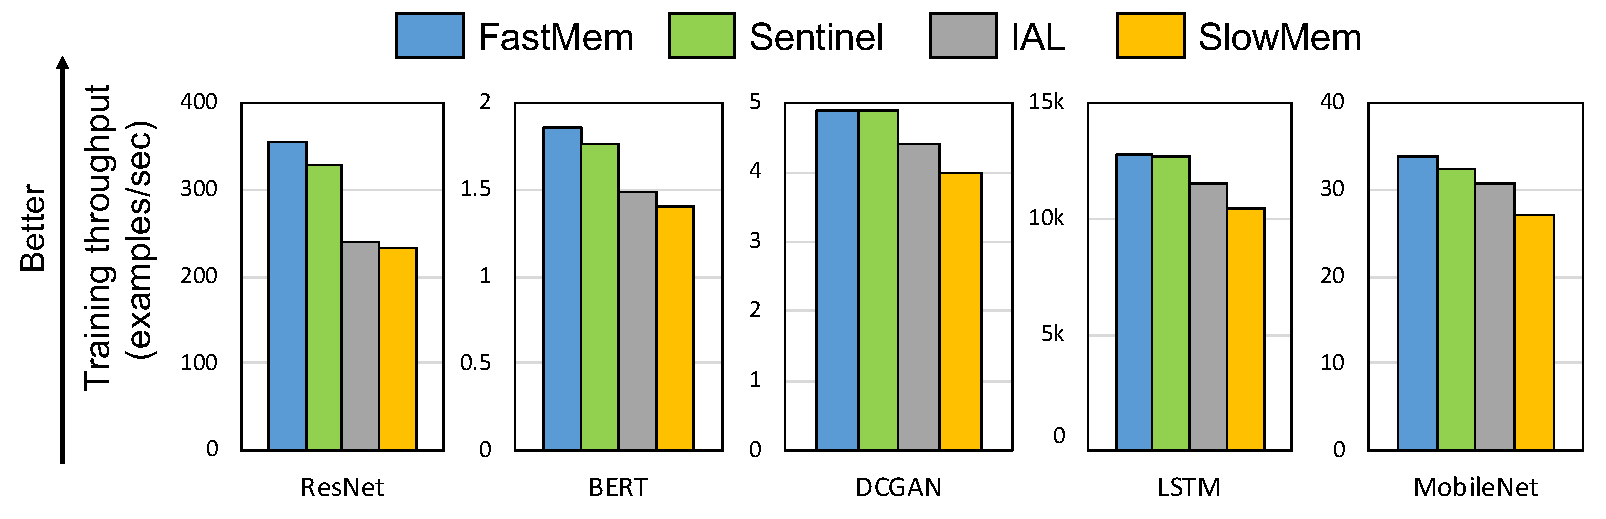
\includegraphics[width=0.48\textwidth]{figures/sentinel_performance.pdf}
\vspace{-20pt}    
\caption{
\textcolor{check}{
Performance with \name, IAL and two configurations. %``RN'' and ``MN'' stand for ``ResNet-32'' and ``MobileNet'' respectively.
}
\vspace{-5pt}
\label{fig:general_perf}}
\end{figure}

%\textcolor{red}{Figure: total number of migrations per model for Sentinel and Nimble.} \textcolor{green}{two bar each subfigure} 
Table~\ref{tab:migration} reports the number of migrations in \name and IAL. Compared with IAL, \name has more migrations \textcolor{check}{(91\% more on average)}. Frequent migrations allow \name to make best use of fast memory for performance. \textcolor{check}{Those migrations are  overlapped with the training process to minimize migration overhead.}
%Also, those migrations are successfully overlapped with DNN training to avoid performance loss. 


\textcolor{check}{\textbf{Memory bandwidth.} 
We analyze memory bandwidth consumption in IAL and \name, shown in Figure~\ref{fig:bandwidth_consumption}. 
%In IAL, most page access happens in slow memory because the migration in IAL is reactive and can not effectively migrate hot pages into fast memory. 
Compared with IAL, \name consumes much higher (multiple times) memory bandwidth in fast memory, indicating that fast memory accesses happen much more often in \name than in IAL. \name also has lower memory bandwidth consumption in slow memory, compared with IAL, indicating that \name reduces accesses in slow memory.} %Figure~\ref{fig:bandwidth_consumption} reveals that \name makes memory accesses in fast memory more often.  }

%\textcolor{jie}{We further analyze the memory bandwidth usage in IAL and \name. Figure~\ref{fig:bandwidth_consumption} shows the read and write memory bandwidth for \name and IAL. In IAL, most page access happens in slow memory because the migration in IAL is reactive and can not effectively migrate hot pages into fast memory. Compared to IAL, \name has much higher read/write bandwidth in fast memory, which indicates that the fast memory access much more often in \name than in IAL. \name also has lower slow memory bandwidth consumption comparing with IAL, which means \name reduces the number of memory access in slow memory. Figure~\ref{fig:bandwidth_consumption} reveals the reason \name outperforms IAL is that \name actively migrates pages and makes pages access happens in fast memory as much as possible. Note that \name migrate pages asynchronously, page access in slow memory may not impact overall performance because the bandwidth is consuming for proactively migrate pages from slow memory to fast memory.} 
%Such reduction comes from reducing unnecessary data movement for short-lived data objects. For some long-lived data objects, test-and-trial also helps to reduce their data movement if the data movement is not helpful for performance. 



\begin{comment}
\begin{table}[]
\small
\caption{\textcolor{jie}{If keep the result?
Number of page migrations in one epoch. ``RN'' and ``MN'' stand for ``ResNet-32'' and ``MobileNet'' respectively.}}
\begin{tabular}{|p{1cm}|p{0.9cm}|p{1cm}|p{1cm}|p{0.9cm}|p{0.9cm}|}
\hline
   & RN(v1) & RN(v2) & DCGAN & LSTM & MN \\ \hline
IAL  & 807308	& 3432254 &	211684	&194933  & 144882 \\ \hline
Sentinel & 2097152	& 4898697	& 444846 &	353500  & 249290 \\ \hline
\end{tabular}
\label{tab:migration}
\end{table}
\end{comment}

%\begin{comment}
\begin{table}[]
\small
\caption{Number of page migrations in one epoch. %``RN'' and ``MN'' stand for ``ResNet-32'' and ``MobileNet'' respectively.
}
\vspace{-5pt}
\begin{tabular}{|p{1.05cm}|p{1cm}|p{0.9cm}|p{1cm}|p{0.9cm}|p{1.1cm}|}
\hline
   & ResNet & BERT & DCGAN & LSTM & MobileNet \\ \hline
\textbf{IAL}  & 807308	& 732540 &	211684	&194933  & 144882 \\ \hline
\textbf{Sentinel} & 2097152	& 1032450	& 444846 &	353500  & 249290 \\ \hline
\end{tabular}
\vspace{-5pt}
\label{tab:migration}
\end{table}
%\end{comment}
\begin{figure}
\centering
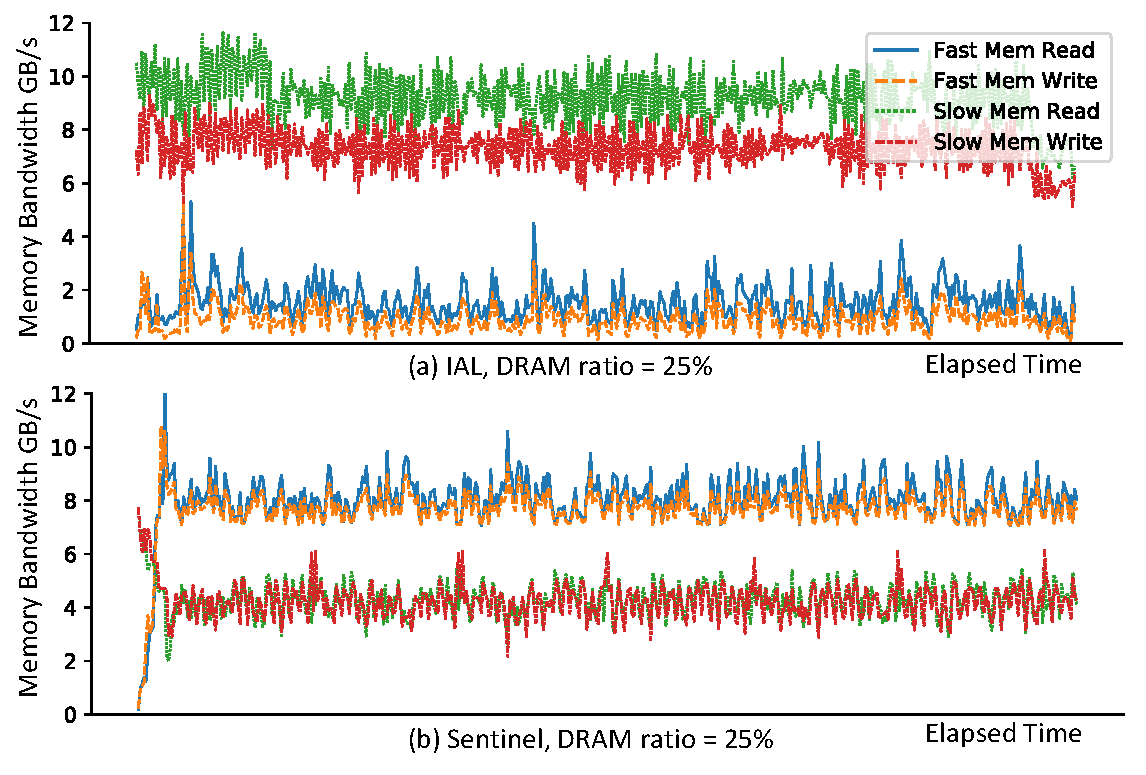
\includegraphics[width=0.48\textwidth]{figures/bandwidth.pdf}
\vspace{-20pt}
\caption{\textcolor{check}{Memory access bandwidth during training of ResNet-32}.}
\vspace{-5pt}
\label{fig:bandwidth_consumption}
\end{figure}


\textcolor{check}{\textbf{Runtime overhead.}% The last column in 
Table~\ref{tab:models} shows the total number of training steps used for profiling, determining migration interval,  and test-and-trail. Those steps have longer execution time than regular training steps, hence introducing runtime overhead. On average, \name uses only 5.6 training steps. Each of those training steps is extended by up to \textcolor{check}{5x} in terms of execution time. However, such overhead is easily amortized by millions of training steps. As a result, the runtime overhead of \name is negligible (less than 1\%).}

%\textcolor{jie}{\textbf{Overhead of \name. }}
%\textcolor{jie}{We discuss the overhead of \name in terms of execution time and memory consumption. The last column in table~\ref{tab:models} shows the total number of training steps used for profiling, determining migration interval and test-and-trail. Comparing with hundreds of thousands of training steps for DNN to converge, \name only uses 5.6 training steps on average to decide an optimal solution for data management. The runtime overhead bring by \name is negligible.}

\textcolor{check}{\textbf{Memory overhead.}
Using our method for data object-level profiling increases peak memory consumption, causing memory overhead. Table~\ref{tab:mem_sentinel} shows peak memory consumption before and after using \name. \name does not increase peak memory consumption much (by 2.1\% at most). This is because data objects larger than one page dominate total memory consumption. Profiling those data objects with \name does not cause memory overhead.}

%Although our profiling method %does not put more than one data objects into the same page for high profiling accuracy, %increases memory consumption, it does not increase much (by 2.1\% at most). This is because data objects larger than 4KB dominate total memory consumption. During the profiling, we do not significantly increase their memory consumption. 

\begin{comment}
\begin{table}[]
\caption{\textcolor{dong}{
Peak memory consumption with and without \name.}}
\centering
%\small
\begin{tabular}{|l|l|l|}
\hline
                & w/o Sentinel & w/ Sentinel \\ \hline
ResNet-32  & 6144 MB& 6176 MB    \\ \hline
BERT & 32760 MB &  34938 MB  \\ \hline
LSTM            & 2048 MB   & 2080 MB            \\ \hline
DCGAN           & 3072 MB   &  3136 MB           \\ \hline
MobileNet       & 4096 MB       &  4228 MB          \\ \hline
\end{tabular}
\label{tab:mem_sentinel}
\end{table}
\end{comment}
%%%%%%%%%%%%%%%%%%%%%%%%%%%%%%%
\begin{table}[]
\caption{\textcolor{check}{
Peak memory consumption with and without \name.}}
\vspace{-5pt}
\small
\begin{tabular}{|p{1.4cm}|p{0.9cm}|p{1cm}|p{1cm}|p{0.9cm}|p{1.1cm}|}
\hline
   & ResNet& BERT & DCGAN & LSTM & MobileNet \\ \hline
w/o Sentinel  & 6144MB	& 32760MB &	3072MB	&2048MB  & 4096MB \\ \hline
w/ Sentinel & 6176MB	& 34938MB	& 3136MB &	2080MB  & 4228MB\\ \hline
\end{tabular}
\vspace{-5pt}
\label{tab:mem_sentinel}
\end{table}
%%%%%%%%%%%%%%%%%%%%%%%%%%%%%%
\begin{figure}[htb!]
	\centering
	%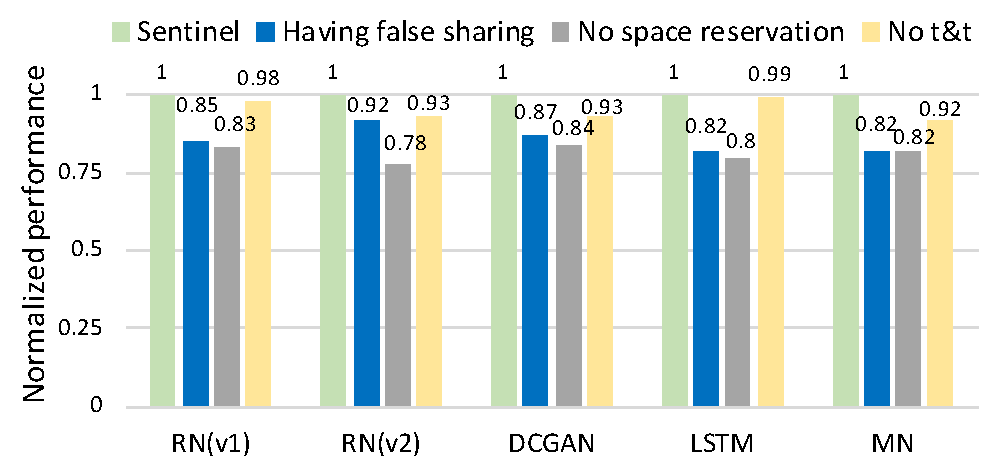
\includegraphics[width=0.48\textwidth]{figures/figure11.pdf}
	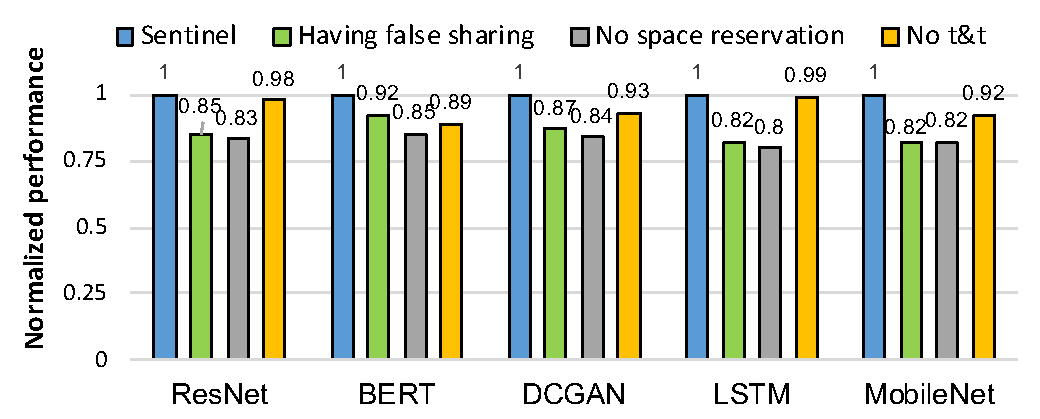
\includegraphics[width=0.48\textwidth]{figures/diff_strategy.pdf}
	\vspace{-20pt}
\caption{\textcolor{check}{
Performance with different strategies for data management in \name. Performance is normalized by that of the full-featured \name.}}
\vspace{-5pt}
\label{fig:fast_memory}
\end{figure}

\textbf{Performance breakdown.}
%%\textcolor{red}{Figure: Multiple strategies, %showing memory pre-allocation, Sentinel without handling false sharing, no preservation space for short-lived variables, test and trail}
%\textcolor{green}{four bars groups together, 5 groups in one figure.} %\textcolor{red}{Figure: show how often the three cases happen at the end of each migration interval.}
We apply different strategies for data management, in order to study the impact of various techniques. Figure~\ref{fig:fast_memory} shows the results. In the figure, we show four strategies: \name without handling page-level false sharing (labeled ``Having false sharing''), \name without reserving fast memory space for short-lived data objects (labeled ``No space reservation''), \name without test-and-trial (labeled ``No t\&t''), and \name with all techniques.

The figure reveals that among the three (handling page-level false sharing, reserving fast memory, and test-and-trial), 
reserving fast memory space for short-lived data objects is the most effective one. We easily have \textcolor{check}{15\% - 20\%} 
%17\% - 23\%
performance loss without it (compared with the full-featured \name). Furthermore, because of the pervasiveness of page-level false sharing, handling false sharing improves performance by \textcolor{check}{8\% - 18\%}.



\begin{figure}[htb!]
	\centering
	%\includegraphics[width=0.9\linewidth,height=0.45\linewidth]{ASPLOS2020_Jie/figures/f11_edit.pdf}
	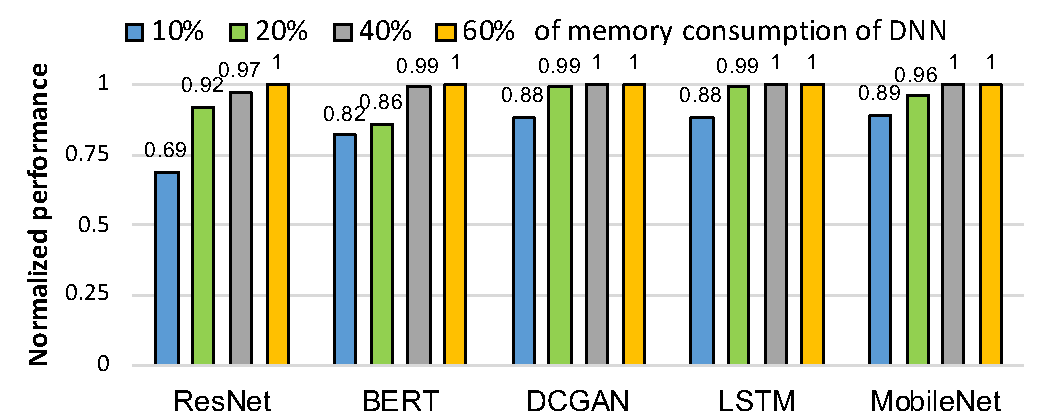
\includegraphics[width=0.48\textwidth]{figures/diff_size.pdf}
	\vspace{-20pt}
\caption{Performance with \name under various sizes of fast memory. The fast memory size is shown as the percentage of peak memory consumption of DNN models. Performance is normalized by that of the fast memory-only.}
\vspace{-5pt}
\label{fig:fast_memory_sen}
\end{figure}

\textbf{Sensitivity study.}
%\textcolor{red}{Figure: sensitivity study: show the effects of fast memory capacity.}
%\textcolor{green}{5 bars groups together, 5 groups in one figure.} 
We change fast memory size and measure performance. Figure~\ref{fig:fast_memory_sen} shows the results. In general, larger fast memory gives better performance. When the fast memory size is 60\% of peak memory consumption, all of DNN models with \name on HM do not have any performance difference from the fast memory-only system. Also, with \name, performance is not sensitive to fast memory size: There is at most 
%8\% 
\textcolor{check}{12\%}
performance variance \textcolor{check}{when fast memory size is changed from 20\% to 40\% of peak memory consumption}. This is a demonstration of how \name effectively uses data movement to make best use of fast memory. 

%\textcolor{red}{Figure: sensitivity study: migration interval} We change the migration interval and study how it impacts the occurrences of the three cases (see Section~\ref{sec:adaptive_dm}): Case 1: all migrations are done (labeled as ``all done''), Case 2: migrations cannot be finished because of no fast memory space (labeled as ``no space'', Case 2: migration cannot be finished because of no time (labeled as ``no time''). Figure~\ref{} shows the results. When the migration interval is large, Case \textcolor{red}{xxx} is more frequent, because \textcolor{red}{xxx}; When the migration is small, Case \textcolor{red}{xxx} is more frequent, because \textcolor{red}{xxx}. 


%\textcolor{red}{Figure: sensitivity study: memory latency and bandwidth}



%\textbf{Cost Saving. TBD}
\textbf{Saving fast memory size.} 
%Figure~\ref{fig:general_perf} shows that using 20\% of peak memory consumption
%peak memory  consumption 
%of DNN models as fast memory size, \name on HM has almost the same performance (8\% difference at most) as the fast memory-only. This brings 80\% saving in fast memory size.
\textcolor{check}{Figure~\ref{fig:general_perf} shows that using 20\%-25\% of peak memory consumption
%peak memory  consumption 
of DNN models as fast memory size, \name on HM has almost the same performance (8\% difference at most) as the fast memory-only. 
This brings over 75\% saving in fast memory size.} 
Figure~\ref{fig:fast_memory_sen} shows that using 60\% of peak memory consumption as fast memory size, there is no performance loss, which comes with 40\% saving in fast memory size.


\begin{figure}
\centering
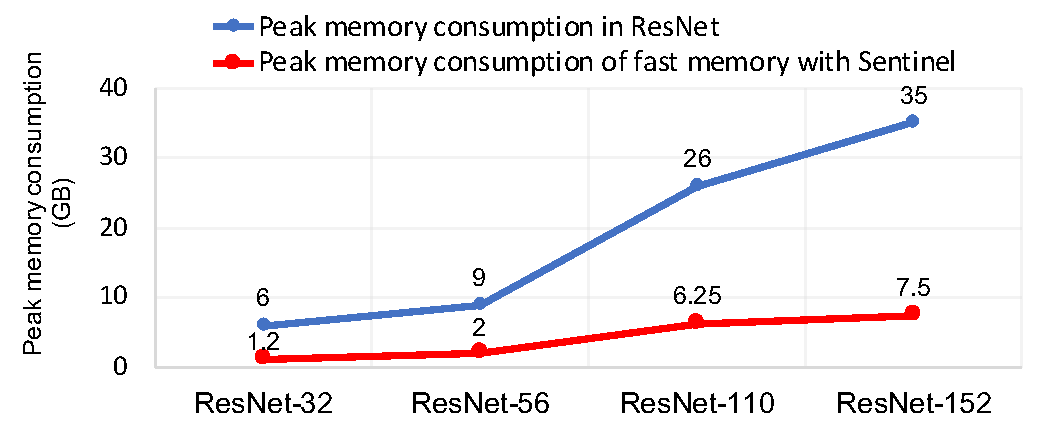
\includegraphics[width=0.48\textwidth]{figures/resnet_diff_input.pdf}
\vspace{-20pt}
\caption{Comparison between peak memory consumption of DNN models and fast memory size for ResNet variants.}
\vspace{-5pt}
\label{fig:mem_consumption}
\end{figure}

%\textcolor{red}{Figure: show the cost saving.}
%\textcolor{green}{two bars in one group. five groups in one figure.}

To further study \name's effectiveness, we use ResNets with various topology and different peak memory consumption. We report the minimum fast memory size with which \name performs the same as the fast memory-only. %\textit{does not have performance loss} with \name, %compared to the fast memory-only cases.
Figure~\ref{fig:mem_consumption} shows peak memory consumption and fast memory size for all ResNet variants. The figure shows that although peak memory consumption increases quickly as ResNet becomes more complicated, the fast memory size increases in a much slower rate. This demonstrates the effectiveness of using \name to save fast memory size.


\begin{comment}
\begin{figure}
\centering
\begin{tikzpicture}
    \begin{axis}[
        width  = 0.5*\textwidth,
        height = 0.3*\textwidth,
        major x tick style = transparent,
        ybar=0.5*\pgflinewidth,
        bar width=10pt,
        %ymajorgrids = true,
        ylabel = {Cost saving},
        symbolic x coords={AA,BB,CC,DD,EE},
        xtick = data,
        scaled y ticks = false,
        enlarge x limits=0.25,
        ymin=0,
        ylabel shift=-0.1cm,
        legend cell align=left,
        legend columns=2,
        legend style={                        at={(1,1.05)},
                anchor=south east,
                column sep=1ex
        }
    ]
        \addplot[style={fill=RYB1,mark=none}]
            coordinates {(AA, 1.0) (BB,1.0) (CC,1.0) (DD,1.0) (EE,1.0)};

        \addplot[style={fill=RYB2,mark=none}]
             coordinates {(AA, 1.0) (BB,1.0) (CC,1.0) (DD,1.0) (EE,1.0)};

        \legend{C1,C2}
    \end{axis}
\end{tikzpicture}
\caption{\textcolor{red}{TODO}}
\end{figure}
\end{comment}
%\textcolor{red}{Figure: number of writes to slow memory for Sentinel and Nimble.}

